\documentclass{article}
\usepackage{graphicx}
\title{title of the document}
\author{name}
\date{August 2024}


\begin{document}
\maketitle

\section{Introduction}
In publishing and graphic design, Lorem ipsum is a placeholder text commonly used to demonstrate the visual form of a document or a typeface without relying on meaningful content. Lorem ipsum may be used as a placeholder before the final copy is available. In publishing and graphic design, Lorem ipsum is a placeholder text commonly used to demonstarte the visual form of a document or a typeface without relying on meaningful content. $h^2 = @6$

% $\%  \$$ \\
% \begin{array}{c}
%     \sigma \\
%     \pi
% \end{array}

\begin{equation}
    \sqrt{5} + \frac{1}{5}\sigma + 5 = a + 2
\end{equation}

\begin{itemize}
    \item first point placeholder text commonly used to demonstarte the visual form of a document or a typeface
    \item second point
    \item third point
\end{itemize}
\begin{enumerate}
    \item first point placeholder text commonly used to demonstarte the visual form of a document or a typeface
    \item second point
    \item third point
\end{enumerate}

Lorem ipsum may be used as a placeholder before the final copy is available

\subsection{graphic}
publishing and graphic design, Lorem ipsum is a placeholder text commonly used to demonstarte the visual form of a document or a typeface without relying on meaningful content. Lorem ipsum may be used as a placeholder before the placeholder text commonly used to demonstarte the visual form of a document or a typeface without relying on meaningful content. Lorem ipsum may be used as a placeholder befor the final

\begin{figure}[h]
    \centering
    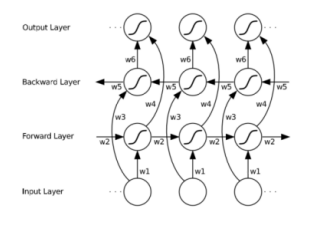
\includegraphics{assets/image1.png}
    \caption{image}
    \label{fig: an image label}
\end{figure}

\subsubsection{graphic2}

copy is available. In publishing and graphic design, Lore ipsum is a place-holder text commonly used to demonstarte the visual form of a document or a typeface without relying on meaningful content. Lorem ipsum may be used as a placeholder bofer the final copy is available.
\begin{table}[h]
    \centering
    \caption{Table Heading}
    \\
    \begin{tabular}{|c|c|c|c|}
        \hline
        \multicolumn{2}{|c|}{First Column} & \multicolumn{2}{c|}{second column}                                 \\
        \hline
        Volley                             & Cricket                       & \multicolumn{2}{c|}{Football} \\
        \hline
        Apple                              & mango                         & \multicolumn{2}{c|}{cherry}   \\
        \hline
    \end{tabular}
\end{table}

\end{document}